\section{klin.med.-grundlagen.txt}

\subsection{Klinische – MedizinMechatronik}
	\begin{itemize}
		\item Dr.med.S.Heidler-Bretterbauer
		\item 
		\item copyright 2014
	\end{itemize}

\subsection{Allgemeine Krankheitslehre}
	\begin{itemize}
		\item Klinische Medizin – Mechatronik
		\item 
		\item Dr.med.S.Heidler-Bretterbauer	copyright 2014
	\end{itemize}

\subsection{Lehrinhalte „klinische Medizin“:}
	\begin{itemize}
		\item allgemeine Grundlagen der Krankheitslehre
		\item häufige Erkrankungen im Detail
		\item Diagnostik
		\item Therapie
	\end{itemize}

\subsection{allgemeine Pathologie}
	\begin{itemize}
		\item Definition
			\begin{itemize}
				\item Pathos, Logos
				\item Lehre von den Krankheiten (ihren Ursachen und den  Veränderungen, die sie im Organismus hervorrufen)
				\item 
			\end{itemize}
		\item Ätiologie:
			\begin{itemize}
				\item Lehre von den Krankheitsursachen
			\end{itemize}
		\item Pathogenese:
			\begin{itemize}
				\item Lehre von der Entstehung einer Krankheit
			\end{itemize}
	\end{itemize}

\subsection{Epidemiologie}
	\begin{itemize}
		\item ursprüngliche Bedeutung: „Seuchenkunde“
		\item WHO Definition:
			\begin{itemize}
				\item die Epidemiologie befasst sich mit der Untersuchung der Verteilung von Krankheiten, physiologischen Variablen und sozialen Krankheitsfolgen in menschlichen Bevölkerungsgruppen sowie mit Faktoren, die diese Verteilung beeinflussen
				\item Begriffsdefinitionen:
					\begin{itemize}
						\item Gesundheit, Krankheit
						\item Morbidität, Mortalität, Letalität
						\item Inzidenz, Prävalenz
					\end{itemize}
		\end{itemize}
	\end{itemize}

\subsection{Epidemiologie}
	\begin{it>emize}
		\item Gesundheit:
			\begin{itemize}
				\item Zustand völligen körperlichen, seelischen und sozialen Wohlbefindens
			\end{itemize}
		\item Krankheit:
			\begin{itemize}
				\item Störung in diesem körperlich-seelisch-	geistig-sozialen Gleichgewicht
			\end{itemize}
		\item Morbidität
			\begin{itemize}
				\item Häufigkeit einer bestimmten Krankheit in einer Bevölkerungsgruppe
				\item Verhältnis der Zahl der Erkrankungen zur Zahl der Gesamtbevölkerung in einem bestimmten Zeitraum
			\end{itemize}
	\end{itemize}

\subsection{Epidemiologie}
	\begin{itemize}
		\item Mortalität („Sterblichkeit“)
			\begin{itemize}
				\item Häufigkeit einer bestimmten Kh als Todesursache in einer Bevölkerungsgruppe
				\item Verhältnis der Zahl der Todesfälle an bestimmter Erkrankung zur Zahl der Gesamtbevölkerung in einem bestimmten Zeitraum, i.d.R. 1 Jahr, pro 100000 Einwohner
				\item 
			\end{itemize}
		\item Letalität („Tödlichkeit“)
			\begin{itemize}
				\item Zahl der Todesfälle bezogen auf die Zahl der Erkrankten
				\item Verhältnis der Zahl der Todesfälle zur Zahl der an einer bestimmten Krankheit Erkrankten („Mortalität in %“)
			\end{itemize}
	\end{itemize}

\subsection{Epidemiologie}
	\begin{itemize}
		\item Inzidenz (= Erkrankungshäufigkeit)
			\begin{itemize}
				\item Zahl von Neuerkrankungen an einer bestimmten KH innerhalb eines bestimmten Zeitraumes
				\item Anzahl der Personen, die im Verlauf eines bestimmten Zeitraumes (i.d.R. 1 Jahr) an einer bestimmten Krankheit erstmals erkranken
			\end{itemize}
		\item Prävalenz
			\begin{itemize}
				\item Zahl der zu einem bestimmten Zeitpunkt an einer bestimmten KH leidenden Personen, bezogen auf die Gesamtbevölkerung
			\end{itemize}
	\end{itemize}

\subsection{Methoden der pathologischen Diagnostik}
	\begin{itemize}
		\item intravitale Diagnostik
			\begin{itemize}
				\item zytologische Untersuchungsmethoden
				\item histologische Untersuchungsmethoden
			\end{itemize}
		\item postmortale Diagnostik
			\begin{itemize}
				\item sanitätspolizeiliche Obduktion
				\item gerichtsmedizinische Obduktion
				\item klinische Obduktion
			\end{itemize}
	\end{itemize}

\subsection{intravitale Diagnostik}
	\begin{itemize}
		\item zytologische Untersuchungsmethoden
			\begin{itemize}
				\item Analyse von Einzelzellen
				\item Gewinnung der Zellen:
					\begin{itemize}
						\item von Schleimhautoberflächen, Sekreten, Spülflüssigkeiten
						\item durch Punktion von Flüssigkeiten
						\item durch Feinnadelpunktion von Organen
					\end{itemize}
				\item Zweck / häufige Fragestellungen:
					\begin{itemize}
						\item infektiöse Erkrankungen (Erregernachweis) und deren Folgen
						\item Entzündungsdiagnostik
						\item Tumorzellnachweis, etc.
					\end{itemize}
			\end{itemize}
	\end{itemize}

\subsection{intravitale Diagnostik}
	\begin{itemize}
		\item histologische Untersuchungsmethoden
			\begin{itemize}
				\item Analyse von Gewebeschnitten von chirurgisch oder bioptisch gewonnenen Gewebestücken
				\item Gefrierschnellschnitt, Paraffinschnitt
				\item Analysetechniken:
					\begin{itemize}
						\item Lichtmikroskopie:
							\begin{itemize}
								\item Anfertigung von Paraffinschnitten oder Gefrierschnitten
							\end{itemize}
						\item Immunfluoreszenz
						\item Elektronenmikroskopie
					\end{itemize}
		\item Zweck / häufige Fragestellungen:
			\begin{itemize}
				\item Zellbeurteilung im Gewebeverband, Tumordiagnostik, Kontrolle des chirurgischen Eingriffs (Resektionsränder), etc.
			\end{itemize}
		\end{itemize}
	\end{itemize}

\subsection{No Title}
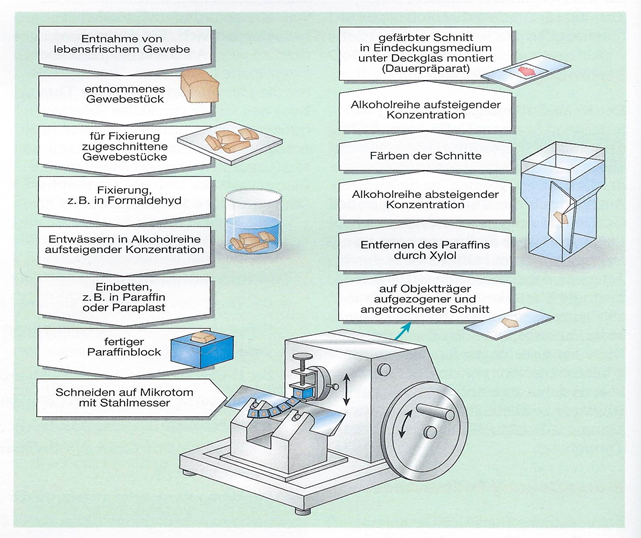
\includegraphics{klin.med.-grundlagen-img0000.png}

\subsection{intravitale Diagnostik}
	\begin{itemize}
		\item bakteriologische und serologische Diagnostik
			\begin{itemize}
				\item mikroskopischer Nachweis von Krankheitserregern
					\begin{itemize}
						\item spezielle Färbemethoden zur Darstellung der Mikroorganismen
							\begin{itemize}
								\item Lichtmikroskopie
								\item Elektronenmikroskopie
							\end{itemize}
						\item kultureller Nachweis von Krankheitserregern
							\begin{itemize}
								\item Bakterienkultur auf flüssigen oder festen Nährmedien
							\end{itemize}
						\item serologischer Nachweis von Krankheitserregern
							\begin{itemize}
								\item Antigen-Antikörper-Reaktion
								\item Agglutinationsreaktionen
									\begin{itemize}
										\item Antigen-Suchtest
										\item Antikörper-Suchtest
									\end{itemize}
								\item 
							\end{itemize}
					\end{itemize}
			\end{itemize}
	\end{itemize}

\subsection{intravitale Diagnostik}
	\begin{itemize}
		\item Spezialmethoden
			\begin{itemize}
				\item Elektronenmikroskopie
				\item Immunhistochemie
					\begin{itemize}
						\item Sichtbarmachen spezieller Zell- und Gewebe-Strukturen durch spezifische AG-AK-Reaktionen mittels monoklonaler AK
					\end{itemize}
				\item biochemische Untersuchungen
					\begin{itemize}
						\item Nachweis bestimmter Strukturen aus Körperflüssigkeiten
						\item Techniken: Immuno-Assay, Blotting-Verfahren (Immunoblot)
					\end{itemize}
				\item molekularbiologische Techniken
					\begin{itemize}
						\item Hybridisierungsmethoden
						\item Amplifizierungsmethoden
					\end{itemize}
		\end{itemize}
	\end{itemize}

\subsection{postmortale Diagnostik}
	\begin{itemize}
		\item Obduktion, Sektion, innere Leichenbeschau, Autopsie:
		\item sanitätspolizeiliche Obduktion:
			\begin{itemize}
				\item bei ungenügender Information
			\end{itemize}
		\item gerichtsmedizinische Obduktion:
			\begin{itemize}
				\item bei Verdacht auf Fremdverschulden
			\end{itemize}
		\item klinische Obduktion:
			\begin{itemize}
				\item zur Qualitätskontrolle
			\end{itemize}
		\item Zweck:
			\begin{itemize}
				\item Grundlage für Statistiken und gesundheitspolitische Maßnahmen
				\item wissenschaftliche Aufgaben
				\item rechtliche Grundlagen siehe Krankenanstaltengesetz
			\end{itemize}
	\end{itemize}

\subsection{Übersicht:Krankheitsursachen, -Verlauf, -Ausgang}
	\begin{itemize}
		\item Krankheitsursachen (Ätiologie)
			\begin{itemize}
				\item endogene Krankheitsursachen
				\item exogene Krankheitsursachen
			\end{itemize}
		\item Krankheitsverlauf
			\begin{itemize}
				\item nach zeitlichem Verlauf
				\item Rezidiv, Remission
			\end{itemize}
		\item Krankheitsausgang
	\end{itemize}

\subsection{Krankheitsursachen}
	\begin{itemize}
		\item innere (endogene) Krankheitsursachen:
			\begin{itemize}
				\item genetische Störungen:
					\begin{itemize}
						\item Chromosomenschäden, DNA-Schäden
					\end{itemize}
				\item Disposition:
					\begin{itemize}
						\item Altersdisposition, Geschlechtsdisposition, genetische Disposition, patholog. Disposition
					\end{itemize}
				\item Autoimmunerkrankungen
				\item hormonelle (endokrine) Störungen
			\end{itemize}
	\end{itemize}

\subsection{Krankheitsursachen}
	\begin{itemize}
		\item äußere (exogene) Krankheitsursachen:
		\item Noxen
			\begin{itemize}
				\item eine Noxe ist eine Substanz oder ein Ereignis, das einem biologischen Organismus Schäden zufügt
				\item im weiteren Sinn versteht man unter einer "Noxe" jede Art von äußerer Krankheitsursache
			\end{itemize}
	\end{itemize}

\subsection{Krankheitsursachen - Noxen}
	\begin{itemize}
		\item physikalische Noxen
			\begin{itemize}
				\item mechanische Einwirkung:
					\begin{itemize}
						\item akut: Trauma (Quetschung, Schnitt, Druck: Barotrauma, …..)
						\item chronisch: Dekubitus
					\end{itemize}
				\item thermische Einwirkung:
					\begin{itemize}
						\item Verbrennungen, Erfrierungen
					\end{itemize}
				\item Luftdruckveränderungen:
					\begin{itemize}
						\item Höhenkrankheit, Dekompressionssyndrom
					\end{itemize}
				\item Stromeinwirkung:
					\begin{itemize}
						\item Verbrennung, Herzrhythmusstörung, Atemlähmung
					\end{itemize}
				\item Strahleneinwirkung:
					\begin{itemize}
						\item UV-Strahlen, ionisierende Strahlung
					\end{itemize}
			\end{itemize}
	\end{itemize}

\subsection{Krankheitsursachen - Noxen}
	\begin{itemize}
		\item biologische Noxen
			\begin{itemize}
				\item lebende Krankheitserreger: Bakterien, Viren, Pilze, Würmer, …
				\item Toxine von Bakterien, Pilzen, Pflanzen, Tieren
			\end{itemize}
		\item chemisch-toxische Noxen
			\begin{itemize}
				\item Laugen oder Säuren
				\item anorganische Verbindungen: Metalle, Staube, Gase
				\item organische Verbindungen: Alkohol, aromatische Amine, …
			\end{itemize}
		\item fehlerhafte Nahrungszufuhr und/oder – verwertung:
			\begin{itemize}
				\item Menge, Zusammensetzung, Aufnahme, ...
			\end{itemize}
		\item psychosoziale Faktoren (Noxe = ?)
	\end{itemize}

\subsection{Krankheitsverlauf}
	\begin{itemize}
		\item perakut:
			\begin{itemize}
				\item besonders rasch, heftig, oft lebensbedrohlich
				\item foudroyant (oder: fulminant) = "blitzartig" einsetzend und verlaufend
			\end{itemize}
		\item akut:
			\begin{itemize}
				\item plötzlicher Beginn, ausgeprägte Symptome (z.B. Lungenembolie)
			\end{itemize}
		\item subakut
			\begin{itemize}
				\item allmählicher Beginn (z.B. Hepatitis B)
			\end{itemize}
		\item chronisch:
			\begin{itemize}
				\item schleichender, längerer Verlauf, Symptome weniger ausgeprägt (z.B. MS)
			\end{itemize}
	\end{itemize}

\subsection{Krankheitsverlauf}
	\begin{itemize}
		\item rezidivierend: wiederkehrend
		\item Rezidiv:
			\begin{itemize}
				\item Wiederauftreten der selben KH nach völliger Abheilung oder nach symptomfreiem Intervall
			\end{itemize}
		\item Remission:
			\begin{itemize}
				\item Zeitspanne der klinischen Symptomfreiheit einer in Schüben verlaufenden Erkrankung
			\end{itemize}
	\end{itemize}

\subsection{Krankheitsausgang}
	\begin{itemize}
		\item Heilung :
			\begin{itemize}
				\item Restitutio ad integrum = völlige Wiederherstellung
			\end{itemize}
		\item Defektheilung :
			\begin{itemize}
				\item Reparatio = bleibender Defekt
				\item z.B. Ersatz durch minderwertiges Narbengewebe
			\end{itemize}
		\item Tod
			\begin{itemize}
				\item die genaue Grenze zwischen Leben und Tod ist schwer zu definieren
				\item so können Patienten mit Herzstillstand manchmal erfolgreich wiederbelebt werden
				\item einzelne Zellen und Gewebe können noch viele Stunden nach eingetretenem Hirntod auf äußere Einflüsse reagieren
			\end{itemize}
	\end{itemize}

\subsection{Tod}
\begin{itemize}
\item klinischer Tod:
\begin{itemize}
\item völliger Kreislaufstillstand; durch Reanimation aufhebbar, solange Funktion des ZNS noch erhalten (Wiederbelebungszeit)
\item unsichere Todeszeichen
\end{itemize}
\item biologischer Tod:
\begin{itemize}
\item Aufhören aller Organ- und Zellfunktionen
\item sichere Todeszeichen
\end{itemize}
\item Hirntod:
\begin{itemize}
\item irreversibler Ausfall aller Hirnfunktionen    Transplantationschirurgie
\item objektive Feststellung: Nulllinien-EEG etc.
\end{itemize}
\end{itemize}

\subsection{Todeszeichen}
\begin{itemize}
\item unsichere Todeszeichen
\begin{itemize}
\item Blässe der Haut und Abkühlung
\item Aufhören der Atemfunktion und der Herz-Kreislauf-Funktion
\begin{itemize}
\item fehlende Atmung
\item fehlender Puls
\item fehlender Herzschlag
\end{itemize}
\item Aufhören der ZNS-Funktion
\begin{itemize}
\item Bewusstlosigkeit
\item fehlender Pupillenreflex (vgl. Areflexie)
\item komplette Lähmung aller Muskeln
\end{itemize}
\end{itemize}
\end{itemize}

\subsection{Todeszeichen}
\begin{itemize}
\item sichere Todeszeichen
\begin{itemize}
\item Verletzungen, die mit dem Leben nicht mehr vereinbar sind (z.B. Fehlen des Kopfes)
\item Totenkälte (Algor mortis)
\item Totenflecken (Livores)
\item Totenstarre (Rigor mortis, Leichenstarre)
\item Autolyse (Verwesung) und Fäulnis
\end{itemize}
\end{itemize}

\subsection{Zellschäden - gewebeschäden}
\begin{itemize}
\item Klinische Medizin – Mechatronik
\item 
\item Dr.med.S.Heidler-Bretterbauer	copyright 2014
\end{itemize}

\subsection{Übersicht}
\begin{itemize}
\item Regeneration – Reparation
\item Zellschäden
\begin{itemize}
\item Ursachen
\item reversible Zellschäden
\begin{itemize}
\item Dystrophie
\end{itemize}
\item irreversible Zellschäden
\begin{itemize}
\item Apoptose
\item Nekrose
\end{itemize}
\item Zellwachstumsstörungen
\begin{itemize}
\item quantitative Zellwachstumsstörungen
\item qualitative Zellwachstumsstörungen
\end{itemize}
\end{itemize}

\subsection{Regeneration - Reparation}
\begin{itemize}
\item Ersatz von verlorengegangenen Zellen oder Geweben durch Zell- und Gewebsneubildung
\item physiologische Regeneration
\begin{itemize}
\item Zellersatz von durch natürlichen Verschleiß verlorengegangenen Zellen
\item die ursprüngliche Struktur und Funktion bleibt erhalten
\end{itemize}
\item pathologischer Gewebeersatz
\begin{itemize}
\item Ersatz von Geweben, die durch krankhafte Einflüsse zugrunde gegangen sind
\begin{itemize}
\item vollständige pathologische Regeneration: Ersatz defekter Zellen und Gewebe durch morphologisch gleichartige und funktionell gleichwertige Strukturen
\item Reparation: Ersatz durch Ersatzgewebsbildung (Defektheilung)
\end{itemize}
\end{itemize}
\end{itemize}

\subsection{Regeneration - Reparation}
\begin{itemize}
\item proliferatives Potential von Geweben und Zellen
\begin{itemize}
\item Wechselgewebe = labiles Gewebe
\begin{itemize}
\item Häute/Schleimhäute (Epithel)
\item Knochenmark
\end{itemize}
\item ruhendes = stabiles Gewebe
\begin{itemize}
\item Parenchymzellen, z.B. Leber, Pankreas
\item Mesenchymzellen, z.B. Fibroblasten, glatte Muskelzellen, Chondrozyten, Osteozyten, Endothelien
\end{itemize}
\item permanentes Gewebe
\begin{itemize}
\item Neurone
\item Skelettmuskulatur
\item Herzmuskel
\end{itemize}
\end{itemize}
\end{itemize}

\subsection{Ursachen des Zellschadens (Noxen)}
\begin{itemize}
\item Hypoxie (   hypoxische Zellschädigung)
\begin{itemize}
\item häufigster Mechanismus einer Zellschädigung
\item Mangeldurchblutung durch Hypotonie, Arteriosklerose, Thrombose, ….
\end{itemize}
\item chemische Substanzen
\begin{itemize}
\item toxische Wirkung konzentrationsabhängig, sehr breites Spektrum potentieller Noxen und Angriffspunkte an der Zelle
\end{itemize}
\item Infektion
\begin{itemize}
\item Viren, Bakterien, Pilze, Parasiten mit sehr verschiedenen meist gut definierten zellulären Schädigungsmechanismen (DNA-Schädigung, Toxinwirkung, Immunreaktion)
\end{itemize}
\end{itemize}
\end{itemize}

\subsection{Ursachen des Zellschadens}
\begin{itemize}
\item Immunreaktionen
\begin{itemize}
\item Erregerabwehr (v.a. virale Infektionen), Autoimmunerkrankungen, Transplantatabstoßung
\end{itemize}
\item genetische Defekte
\begin{itemize}
\item führen zu komplexen Multiorganstörungen (z.B. Trisomien)  oder pathogenen Veränderungen einzelner Proteine durch Punktmutationen (z.B. Sichelzellanämie)
\end{itemize}
\item inadäquate Ernährung
\begin{itemize}
\item klassischerweise Mangelernährung (z.B. Vitamine)
\item in Industrienationen aber auch Überangebot, vor allem an Lipiden und Kohlehydraten
\end{itemize}
\item physikalische Einwirkungen
\begin{itemize}
\item mechanische Traumen, Temperatur, Strom,  nichtionisierende (UV) und ionisierende (Röntgen, Radioaktivität) Strahlung
\end{itemize}
\end{itemize}
\end{itemize}

\subsection{Zell- und Gewebereaktionen auf Noxen}
\begin{itemize}
\item Zellschäden
\begin{itemize}
\item reversibel: „Dystrophie“
\item irreversibel: Nekrose, Apoptose
\end{itemize}
\item quantitative Differenzierungsstörung (meist Anpassungsreaktion)
\begin{itemize}
\item Agenesie, Aplasie, Hypoplasie
\item Atrophie
\item Hypertrophie, Hyperplasie
\end{itemize}
\item qualitative Differenzierungsstörung
\begin{itemize}
\item Metaplasie
\item Dysplasie
\item Anaplasie
\end{itemize}
\end{itemize}

\subsection{reversible Zellschädigungen}
\begin{itemize}
\item reversible Zellschädigungen    „point of no return“    irreversible Zellschädigung (Zelltod)
\item Quantität der Noxe entscheidend
\item reversible Zellschädigungen: „Dystrophien“
\begin{itemize}
\item Zellödem („ trübe Schwellung“)
\item intrazelluläre Verfettung (fettige Dystrophie)
\item hyaline Dystrophie / Degeneration
\end{itemize}
\end{itemize}

\subsection{irreversible Zellschädigungen}
\begin{itemize}
\item irreversible Zellschädigungen
\begin{itemize}
\item Apoptose
\item Nekrose
\begin{itemize}
\item Kennzeichen der Nekrose
\item Nekroseformen
\item Folgen der Nekrose
\end{itemize}
\end{itemize}
\end{itemize}

\subsection{Apoptose}
\begin{itemize}
\item Apoptose = programmierter Zelltod
\begin{itemize}
\item genetisch fixiertes „Selbstmordprogramm“ einer Zelle
\item Programm zur Elimination einzelner Zellen deren Funktion nicht mehr benötigt wird oder die einen irreparablen (genetischen) Schaden erlitten haben
\item kann von außen angeregt (extrinisisch) oder durch  zellinterne Mechanismen (intrinsisch) initiiert werden
\item aktiver streng gesteuerter Prozess durch den sichergestellt wird, dass die betroffene Zelle ohne Schädigung des Nachbargewebes zugrundegeht
\item typische Veränderungen:
\begin{itemize}
\item Kernschrumpfung, Zellorganellen und Zellkontakte lösen sich auf
\end{itemize}
\end{itemize}
\end{itemize}
\end{itemize}
\end{itemize}

\subsection{Apoptose}
\begin{itemize}
\item Apoptose als genetisch programmiertes, geregeltes Absterben von Zellen (physiologische Form des Zelltodes):
\begin{itemize}
\item während der Embryonalentwicklung
\item während des Lebens und Alterns
\end{itemize}
\item Apoptose als induziertes Absterben der Zellen:
\begin{itemize}
\item Effekt eines Virusbefalls, einer Immunreaktion oder von Zytokinen, …
\end{itemize}
\end{itemize}

\subsection{Nekrose}
\begin{itemize}
\item Nekrose = provozierter Zelltod
\begin{itemize}
\item Endstrecke einer irreversiblen Stoffwechselstörung
\item passiver Prozess, die Zelle versucht jedoch zuerst durch eine Anpassungsreaktion der Schädigung zu entgehen
\item typische Veränderungen:
\begin{itemize}
\item Zytoplasmaveränderungen (Eosinophilie des Plasmas)
\item Zellkernveränderungen (Karyolyse → Diagnostik!)
\item Zerstörung der Zellmembran mit Übertritt von intrazellulären Enzymen in die Umgebung und ins Blut
\item Reaktion des umgebenden Gewebes:
\end{itemize}
\item hyperämischer Randsaum
\item leukozytärer Demarkationswall
\item Granulationsgewebe
\end{itemize}
\end{itemize}
\end{itemize}
\end{itemize}

\subsection{Nekrose}
\begin{itemize}
\item Nekroseformen:
\begin{itemize}
\item Koagulationsnekrose
\item Kolliquationsnekrose
\item käsige Nekrose
\item gangränöse Nekrose
\item hämorrhagische Nekrose
\end{itemize}
\item Folgen der Nekrose:
\begin{itemize}
\item restitutio ad integrum
\item Defektheilung / Narbenbildung
\item Hohlraumbildung (Zyste etc.)
\item Ulkusbildung
\end{itemize}
\end{itemize}
\end{itemize}

\subsection{Übersicht: Zellwachstumsstörungen}
\begin{itemize}
\item pathologisches Zellwachstum
\begin{itemize}
\item quantitative Wachstumsstörungen
\begin{itemize}
\item Verminderung des Zellwachstums = Atrophie
\item angeborene Störungen mit Hemmung des Wachstums
\item Vermehrung des Zellwachstums = Hypertrophie, Hyperplasie
\end{itemize}
\item qualitative Zellwachstumsstörungen
\begin{itemize}
\item Metaplasie, Dysplasie, Anaplasie
\end{itemize}
\end{itemize}
\end{itemize}

\subsection{Anpassungsreaktionen auf zellulären Stress}

\subsection{quantitative Wachstumsstörungen}
\begin{itemize}
\item Atrophie = Verminderung des Zellwachstums
\begin{itemize}
\item Verkleinerung eines primär normal entwickelten und normal großen Gewebes bzw. Organs
\item Überwiegen der katabolen über die anabolen Stoffwechselvorgänge
\begin{itemize}
\item einfache Atrophie: Zellverkleinerung
\item numerische Atrophie: Verminderung der Zellzahl
\end{itemize}
\item physiologische Atrophie:
\begin{itemize}
\item im Rahmen normaler physiologischer Entwicklungsprozesse
\end{itemize}
\item pathologische Atrophie:
\begin{itemize}
\item im Rahmen krankhafter Ereignisse, Überwiegen der katabolen Prozesse
\end{itemize}
\end{itemize}
\end{itemize}

\subsection{quantitative Wachstumsstörungen}
\begin{itemize}
\item lokale Atrophien
\begin{itemize}
\item auf ein Organ oder einen Gewebsabschnitt beschränkt
\begin{itemize}
\item Inaktivitätsatrophie
\item vaskuläre Atrophie → Ischämie
\item mechanische Druckatrophie → Kompression
\item neurogene Atrophie (fehlende Innervation)
\item Erschöpfungsatrophie
\item endokrine Atrophie (mangelnder hormoneller Stimulus)
\item genetisch bedingte Atrophie
\end{itemize}
\item generalisierte Atrophien
\begin{itemize}
\item den gesamten Körper betreffend
\begin{itemize}
\item senile Atrophie
\item Hungeratrophie
\item Kachexie
\end{itemize}
\end{itemize}
\end{itemize}

\subsection{quantitative Wachstumsstörungen}
\begin{itemize}
\item angeborene Störungen mit Hemmung des Wachstums
\begin{itemize}
\item Agenesie: gesamte Organanlage fehlt
\item Aplasie: Organentwicklung fand nicht statt
\item Hypoplasie: Organentwicklung kam vorzeitig zum Stillstand (Unterentwicklung)
\end{itemize}
\end{itemize}

\subsection{quantitative Wachstumsstörungen}
\begin{itemize}
\item Hypertrophie
\begin{itemize}
\item Organvergrößerung durch Zellvergrößerung ohne Zellvermehrung
\item Steigerung der Leistungsfähigkeit, jedoch Verminderung der Reserve
\begin{itemize}
\item Arbeitshypertrophie (vermehrte Arbeitsbelastung)
\item kompensatorische Hypertrophie
\end{itemize}
\end{itemize}
\end{itemize}

\subsection{quantitative Wachstumsstörungen}
\begin{itemize}
\item Hyperplasie
\begin{itemize}
\item Organvergrößerung durch Zellvermehrung
\item regeneratorische Hyperplasie:
\begin{itemize}
\item Reaktion auf Gewebeschädigung mit überschießender Regeneration / Reparation
\end{itemize}
\item Hyperplasien infolge endokriner Störungen:
\begin{itemize}
\item vermehrter Hormonstimulus
\item z.B. Hyperplasie der Prostata, Hyperplasie der Schilddrüse
\end{itemize}
\end{itemize}
\end{itemize}

\subsection{qualitative Wachstumsstörungen}
\begin{itemize}
\item Metaplasie:
\begin{itemize}
\item Ersatz eines ausdifferenzierten Gewebes durch anderes hochdifferenziertes Gewebe
\end{itemize}
\item Dysplasie:
\begin{itemize}
\item meist noch reversible Veränderungen von Zellen durch atypische Regeneration und Verlust der Differenzierungfließender Übergang zur (irreversiblen) Anaplasie
\end{itemize}
\item Anaplasie:
\begin{itemize}
\item irreversible Entdifferenzierung der Zellen und Gewebe mit Verlust der geweblichen Struktur und der Formbesonderheiten der Zellen = Malignität
\end{itemize}
\end{itemize}